\documentclass{article}

\thispagestyle{empty}
\usepackage%[landscape,scale=.95]
{geometry}

\usepackage{amsmath}
\usepackage{fontspec}
\usepackage{unicode-math}
\setmainfont{TeX Gyre Bonum}
\setmathfont{TeX Gyre Bonum Math}

\usepackage{tikz}
\usetikzlibrary{
  matrix,
  matrix.skeleton,
  decorations.pathreplacing,
  calligraphy,
  positioning
}

\usepackage{quadratics}
\usepackage{rationals}
\usepackage{randomquestions}

\ExplSyntaxOn

\tl_new:N \l__quad_tmpa_tl
\tl_new:N \l__quad_tmpb_tl
\seq_new:N \l__quad_tmpa_seq
\seq_new:N \l__quad_tmpb_seq

\NewDocumentCommand \QuadFromRoots { O{x} m m }
{

  \quad_from_roots:nVV {#1} \l__quad_tmpa_tl \l__quad_tmpb_tl
}

\cs_new_protected_nopar:Npn \quad_from_roots:nnn #1#2#3
{
  \seq_clear:N \l__quad_tmpa_seq
  \seq_clear:N \l__quad_tmpb_seq

  \seq_put_right:Ne \l__quad_tmpa_seq
  { {1} {1} {\tl_item:nn {#2} {3}} {1}}
  \seq_put_right:Ne \l__quad_tmpa_seq
  { {0} {\int_eval:n { (-1) * (\tl_item:nn {#2} {1}) }} {\tl_item:Nn {#2} {2}} {1}}

  \seq_put_right:Ne \l__quad_tmpb_seq
  { {1} {1} {\tl_item:nn {#3} {3}} {1}}
  \seq_put_right:Ne \l__quad_tmpb_seq
  { {0} { \int_eval:n { (-1) * (\tl_item:nn {#3} {1}) }} {\tl_item:nn {#3} {2}} {1}}

  \rat_mult_polynomials:NN \l__quad_tmpa_seq \l__quad_tmpb_seq

  \rat_polynomial:Nn \l__quad_tmpa_seq {#1}
}

\cs_generate_variant:Nn \quad_from_roots:nnn {nVV}

\cs_new_protected_nopar:Npn \quad_row:nnn #1#2#3
{
  \(\quad_from_roots:nnn {#1}{#2}{#3}\)
  \&
  \(\rat_to_frac:n {#2}\)
  \&
  \(\rat_to_frac:n {#3}\)
  \&
  \rat_add:Nnn \l__quad_tmpa_tl {#2} {#3}
  \(\rat_to_frac:V \l__quad_tmpa_tl\)
  \&
  \rat_mult:Nnn \l__quad_tmpa_tl {#2} {#3}
  \(\rat_to_frac:V \l__quad_tmpa_tl\)
}

\cs_generate_variant:Nn \quad_row:nnn {nVV}

\NewDocumentCommand\QuadRow { O{x} m m}
{
  \rat_parse:Nn \l__quad_tmpa_tl {#2}
  \rat_parse:Nn \l__quad_tmpb_tl {#3}
  \quad_row:nVV {x} \l__quad_tmpa_tl\l__quad_tmpb_tl
}

\NewDocumentCommand\RandomQuadRow { O{x} m m}
{
  \random_rat_from_range:Nn \l__quad_tmpa_tl {#2}
  \random_rat_from_range:Nn \l__quad_tmpb_tl {#3}
  \quad_row:nVV {x} \l__quad_tmpa_tl\l__quad_tmpb_tl
}

\ExplSyntaxOff


\begin{document}

\vspace*{\fill}

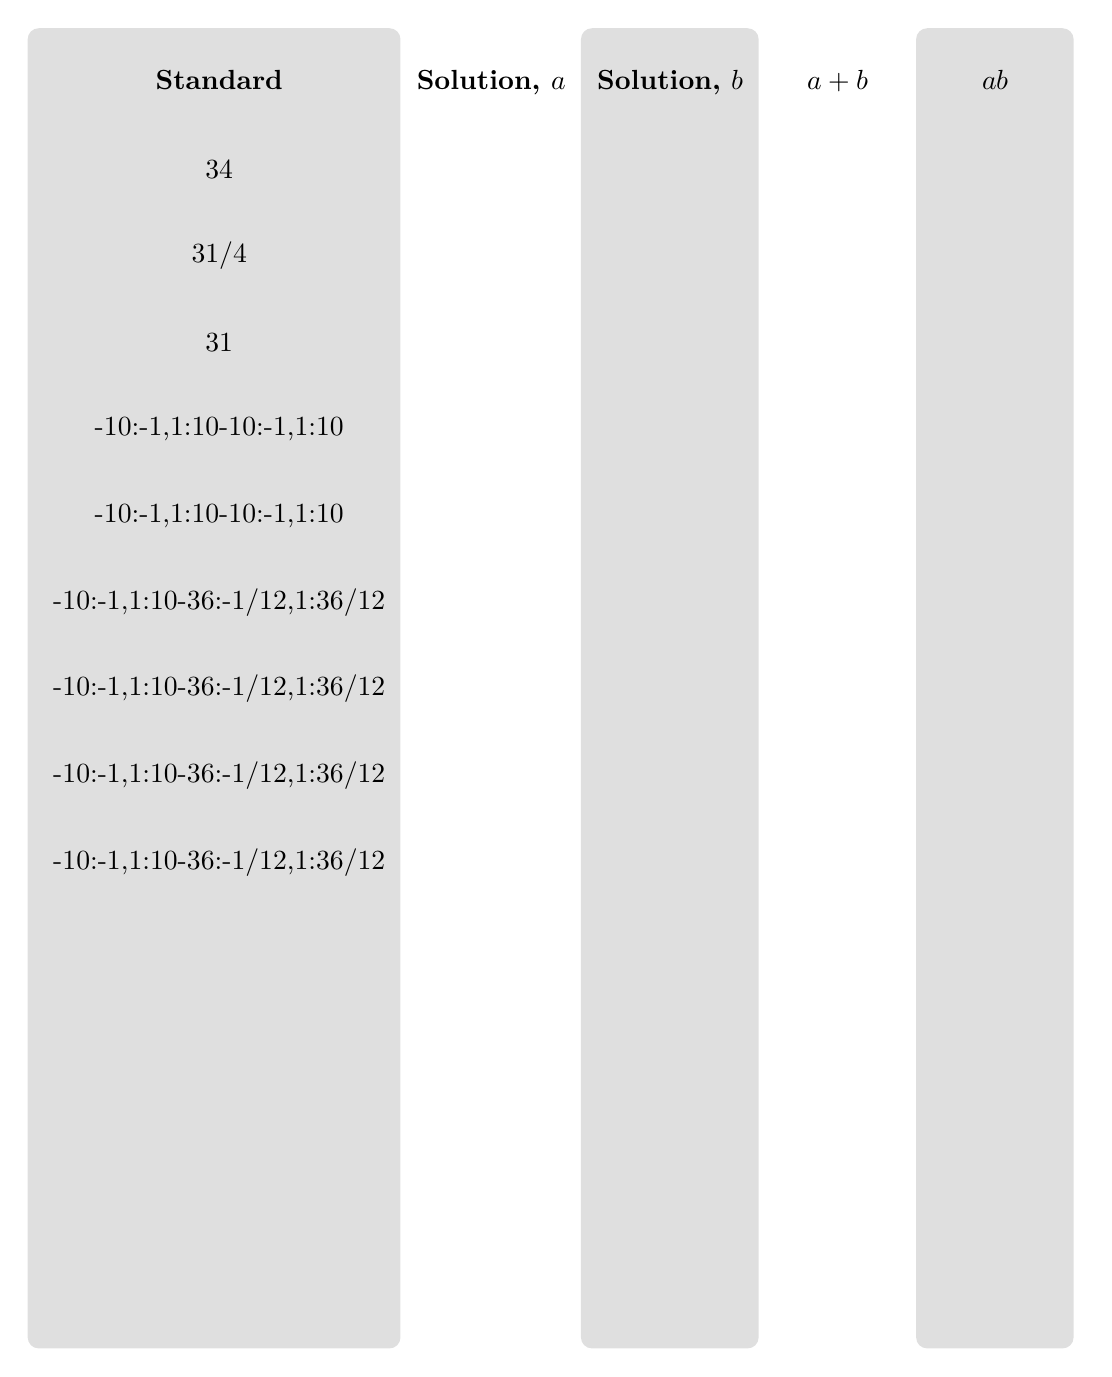
\begin{tikzpicture}
\matrix[
  matrix of nodes,
  ampersand replacement=\&,
  nodes={inner xsep=2mm, minimum width=2cm,text opacity=0,minimum height=1.1cm},
  row 1/.style={every node/.append style={font=\bfseries,text opacity=1}},
  style odd tiling columns={fill=gray!25,rounded corners},
  %
  row 2/.style={every node/.append style={text opacity=1}},
  row 3/.style={every node/.append style={text opacity=1}},
  row 4 column 1/.style={every node/.append style={text opacity=1}},
  row 5 column 1/.style={every node/.append style={text opacity=1}},
  row 6 column 1/.style={every node/.append style={text opacity=1}},
  row 7 column 1/.style={every node/.append style={text opacity=1}},
  row 8 column 1/.style={every node/.append style={text opacity=1}},
  row 9 column 1/.style={every node/.append style={text opacity=1}},
  row 10 column 1/.style={every node/.append style={text opacity=1}},
  row 11 column 2/.style={every node/.append style={text opacity=1}},
  row 11 column 3/.style={every node/.append style={text opacity=1}},
  row 12 column 2/.style={every node/.append style={text opacity=1}},
  row 12 column 4/.style={every node/.append style={text opacity=1}},
  row 13 column 4/.style={every node/.append style={text opacity=1}},
  row 13 column 5/.style={every node/.append style={text opacity=1}},
  row 14 column 2/.style={every node/.append style={text opacity=1}},
  row 14 column 5/.style={every node/.append style={text opacity=1}},
  row 15 column 4/.style={every node/.append style={text opacity=1}},
  row 15 column 5/.style={every node/.append style={text opacity=1}},
  %
]
(m)
{
  Standard \&
  Solution, \(a\) \&
  Solution, \(b\) \&
  \(a + b\) \&
  \(a b\) \&
  \\
  \QuadRow{3}{4} \\
  \QuadRow{3}{1/4} \\
  \QuadRow{3}{1} \\
  \RandomQuadRow{-10:-1,1:10}{-10:-1,1:10} \\
  \RandomQuadRow{-10:-1,1:10}{-10:-1,1:10} \\
  \RandomQuadRow{-10:-1,1:10}{-36:-1/12,1:36/12} \\
  \RandomQuadRow{-10:-1,1:10}{-36:-1/12,1:36/12} \\
  \RandomQuadRow{-10:-1,1:10}{-36:-1/12,1:36/12} \\
  \RandomQuadRow{-10:-1,1:10}{-36:-1/12,1:36/12} \\
  \RandomQuadRow{-10:-1,1:10}{-10:-1,1:10} \\
  \RandomQuadRow{-10:-1,1:10}{-10:-1,1:10} \\
  \RandomQuadRow{-10:-1,1:10}{-10:-1,1:10} \\
  \RandomQuadRow{-10:-1,1:10}{-36:-1/12,1:36/12} \\
  \RandomQuadRow{-10:-1,1:10}{-36:-1/12,1:36/12} \\
};
\end{tikzpicture}

\vspace*{\fill}


\end{document}
